%%%%%%%%%%%%%%%%%%%%%%%%%%%%%%%%%%%%%%%%%%%%%%%%%%%
%
%  Main document template code for TAMU Theses and 
%  Dissertations starting Fall 2016.
%
%  Author:  Kyle R. Wodzicki  
%  Updated: 04 Nov. 2016
%
%  Adapted loosely from: 
%    TAMU LaTeX (SZR) Version 3.16.10 from OGAPS 
%
%%%%%%%%%%%%%%%%%%%%%%%%%%%%%%%%%%%%%%%%%%%%%%%%%%%
\documentclass[12pt]{tamu_thesis}   	% Load the tamu_thesis document class

%%%%%%%%%%%%%%%%%%%%%%%%%%%%%%%%%%%%%%%%%%%%%%%%%%%%
%%%          Load extra packages here            %%%
%%%%%%%%%%%%%%%%%%%%%%%%%%%%%%%%%%%%%%%%%%%%%%%%%%%%
\usepackage[colorlinks=false]{hyperref}	% hyperref with coloring and footnote do NOT get along
\usepackage{multirow}			% Multirow package for tables
\usepackage{footnote}			% Package for the savenotes command
\usepackage{amsthm}				% AMS package for theorems
%\usepackage{natbib,url}			% Load the natbib and ulr packages

%%%%%%%%%%%%%%%%%%%%%%%%%%%%%%%%%%%%%%%%%%%%%%%%%%%%
%%%       Set information for title page.        %%%
%%%%%%%%%%%%%%%%%%%%%%%%%%%%%%%%%%%%%%%%%%%%%%%%%%%%
% Delete or comment out tags that are NOT needed
\Title{The Title of Your Thesis or Dissertation Goes In This Space To Let Us Know What Your Document is About}
\PaperType{Thesis}					% Enter the paper type
\FullName{Aggie D. Student}			% Enter full name
\Degree{Master of Science}			% Enter degree
\Chair{Chair Name}					% Enter name of committee chair
%\CoChair{Co-Chair Name}			% Enter name of committee co-chair
\MemberOne{Committee Member 1}		% Name of first committee member
\MemberTwo{Committee Member 2}		% Name of second committee member
\MemberThree{Committee Member 3}	% Name of third committee member
%\MemberFour{Committee Member 4}	% Name of fourth committee member
\DeptHead{Head of Department}		% Enter name of department head
\GradMonth{December}				% Enter graduation month
\GradYear{2016}						% Enter graduation year
\Dept{Mathematics}					% Enter department name	

%%%%%%%%%%%%%%%%%%%%%%%%%%%%%%%%%%%%%%%%%%%%%%%%%%%%%%
%%%  Set path to the figures and figure extensions %%%
%%%%%%%%%%%%%%%%%%%%%%%%%%%%%%%%%%%%%%%%%%%%%%%%%%%%%%
\graphicspath{ {./graphic/},{./figures/}  }
\DeclareGraphicsExtensions{.png,.PNG,.jpg}

%%%%%%%%%%%%%%%%%%%%%%%%%%%%%%%%%%%%%%%%%%%%%%%%%%%%%%
% Define custom  commands for easier typing        %%%
%%%%%%%%%%%%%%%%%%%%%%%%%%%%%%%%%%%%%%%%%%%%%%%%%%%%%%
\newcommand{\mmday}{mm day$^{-1}$}  % Command for mm day^-1 units


%%%%%%%%%%%%%%%%%%%%%%%%%%%%%%%%%%%%%%%%%%%%%%%%%%%%
%%% Load the nomenclature package. Can set the 'all' 
%%% option to display all. Default is to display 
%%% only the nomenclature/acronyms that are used.
\usepackage[all]{nomenclature}

%%%%%%%%%%%%%%%%%%%%%%%%%%%%%%%%%%%%%%%%%%%%%%%%%%%%
%%%          Beginning of the document           %%%
%%%%%%%%%%%%%%%%%%%%%%%%%%%%%%%%%%%%%%%%%%%%%%%%%%%%
\begin{document}
\maketitle			% Must have this to generate the title page!!!

% Be sure to include all TeX files to be used in your document!
% !TEX root = ../TAMU_Thesis_Main.tex

%%%%%%%%%%%%%%%%%%%%%%%%%%%%%%%%%%%%%%%%%%%%%%%%%%%%%%%%%%%%%%%%%%%%%
%%                           ABSTRACT 
%%%%%%%%%%%%%%%%%%%%%%%%%%%%%%%%%%%%%%%%%%%%%%%%%%%%%%%%%%%%%%%%%%%%%

\begin{abstract}

This is the first numbered page, lower case Roman numberal (ii). Page numbers are outside the prescribed margins, at the bottom of the page and centered; everything else is inside the margins.No bold on this page (Exception: heading ABSTRACT is bold if major headings are bold. \emph{This \LaTeX ~ template applies to this exception}).

Text begins two double spaces below the major heading. Recommended length of text is no more than 350 words. Vertical spacing is double spaced or space-and-a-half. (\emph{This \LaTeX ~ template applies double space for this ABSTRACT.}) The same margin settings and text alignment are followed else where in this thesis. There should be no numbered references or formal citations in ABSTRACT.

The content of this ABSTRACT provides a complete, succinct snapshot of the research, addressing the purpose, methods, results, and conclusions of the research. As a result, it should stand alone without any formal citations or references to chapters/sections of the work. To accomodate with a variety of online database, images or complex equations should also be avoided.

The next pages are Dedication, Acknowledgments, Contributors and Funding Sources, and Nomenclature. Of these, Contributors and Funding Sources is required. The rest are optional.

\end{abstract}			% Include the abstract.tex file
%%%%%%%%%%%%%%%%%%%%%%%%%%%%%%%%%%%%%%%%%%%%%%%%%%%
%
%  New template code for TAMU Theses and Dissertations starting Fall 2016.  
%
%  Author: Sean Zachary Roberson
%	 Version 3.16.09
%  Last updated 9/12/2016
%
%  Modified 04 Nov. 2016 by Kyle R. Wodzicki
%%%%%%%%%%%%%%%%%%%%%%%%%%%%%%%%%%%%%%%%%%%%%%%%%%%

%%%%%%%%%%%%%%%%%%%%%%%%%%%%%%%%%%%%%%%%%%%%%%%%%%%%%%%%%%%%%%%%%%%%%%
%%                           DEDICATION
%%%%%%%%%%%%%%%%%%%%%%%%%%%%%%%%%%%%%%%%%%%%%%%%%%%%%%%%%%%%%%%%%%%%%
\begin{dedication}


\begin{center}
\vspace*{\fill}
To my mother, my father, my grandfather, and my grandmother. To see what happens with multiple lines, I extend this next part into a second line.
\vspace*{\fill}
\end{center}

\end{dedication}			% Include the dedication file
% !TEX root = ../TAMU_Thesis_Main.tex

%%%%%%%%%%%%%%%%%%%%%%%%%%%%%%%%%%%%%%%%%%%%%%%%%%%%%%%%%%%%%%%%%%%%%%
%%                           ACKNOWLEDGMENTS
%%%%%%%%%%%%%%%%%%%%%%%%%%%%%%%%%%%%%%%%%%%%%%%%%%%%%%%%%%%%%%%%%%%%%
\begin{acknowledgements}

This section is also optional, limited to four pages. It must follow the Dedication Page (or Abstract, if no Dedication). If listing preliminary pages in Table of Contents, include Acknowledgments. Heading (\MakeUppercase{Acknowledgments}) is bold if major headings are bold. It should be in same type size and style as text. So does vertical spacing, paragraph style, and margins. Also, ensure that the spelling of ``acknowledgments'' matches throughout the text and the table of contents.

I would like to thank the Texas A\&M University Office of Graduate and Professional Studies to allow me to construct this \LaTeX\ thesis template. Special thanks to JaeCee Crawford, Amy Motquin, Ashley Schmitt, Rachel Krolczyk, and Roberta Caton for carefully reviewing this material.  % use A\&M instead of A$\&$M, not use $A\&M$ as well, the last one won't be bold.


\end{acknowledgements}	% Include the acknowledgements file
% !TEX root = ../TAMU_Thesis_Main.tex

%%%%%%%%%%%%%%%%%%%%%%%%%%%%%%%%%%%%%%%%%%%%%%%%%%%%%%%%%%%%%%%%%%%%%%
%%             CONTRIBUTORS AND FUNDING SOURCES
%%%%%%%%%%%%%%%%%%%%%%%%%%%%%%%%%%%%%%%%%%%%%%%%%%%%%%%%%%%%%%%%%%%%%

\begin{contributors}

%This section is taken directly from the MS Word templates.

%Old version below.

%All theses and dissertations must include a contributors and funding sources section. In this section, name all members of the dissertation committee, and any collaboration with others in carrying out your thesis or dissertation research. Your independent contributions must be made clear.
%
%If financial support from the university or any other source was gained to conduct your thesis or dissertation research and compilation, it must be listed in this section. If you completed all work independently without outside financial support, indicate this here.
%\textit{(Sample Wording)}
%
%This work was supported by a dissertation committee consisting of Professor XXX [advisor – also note if co-advisor] and XXXX of the Department of [Home Department] and Professor(s) XXXX of the Department of [Outside Department].
% 
%The data analyzed for Chapter III was provided by Professor XXXX. The analyses depicted in Chapter IV were conducted in part by Rebecca Jones of the Department of Biostatistics and were published in (year) in an article listed in the Biographical Sketch. 
%
%All other work conducted for the dissertation was completed by the student independently.
%
%\noindent \textit{(or)}
%
%This work was supervised by a dissertation committee consisting of Professor XXXX [advisor – also note if co-advisor] and Professor(s) XXXX of the Department of [Home Department] and Professor(s) XXXX of [Outside Department]. All work for the dissertation was completed independently by the student.
%
%\noindent \textit{(or)}
%
%Graduate study was supported by a fellowship from Texas A\&M University and a dissertation research fellowship from XXX Foundation.

\subsection*{Contributors}
This work was supported by a thesis (or) dissertation committee consisting of Professor XXXX [advisor --– also note if co-advisor] and XXX of the Department of [Home Department] and Professor(s) XXXX of the Department of [Outside Department].

The data analyzed for Chapter X was provided by Professor XXXX. The analyses depicted in Chapter X were conducted in part by Rebecca Jones of the Department of Biostatistics and were published in (year) in an article listed in the Biographical Sketch.

All other work conducted for the thesis (or) dissertation was completed by the student independently.
\subsection*{Funding Sources}
Graduate study was supported by a fellowship from Texas A\&M University and a dissertation research fellowship from XXX Foundation. 

\end{contributors}		% Include the contributors file
\makeNomenclature					% Generate nomenclature if using the nomenclature package

\makeToC							% Generate the Table of Contents. REQUIRED!!!
% !TEX root = ../TAMU_Thesis_Main.tex

%%%%%%%%%%%%%%%%%%%%%%%%%%%%%%%%%%%%%%%%%%%%%%%%%%%%%%%%%%%%%%%%%%%%%%
%%                           SECTION I
%%%%%%%%%%%%%%%%%%%%%%%%%%%%%%%%%%%%%%%%%%%%%%%%%%%%%%%%%%%%%%%%%%%%%

\chapter{Introduction and Literature Review}

\section{Author's Message to the Student Using This Template For Their Thesis or Dissertation}

Howdy! This is the template for theses and dissertations written using \LaTeX for submission at Texas A\&M University. While the \ac{OGAPS} is here to guide you in submitting your thesis or dissertation. This template shows the many features of \LaTeX, with many more available to the user.

Please note that this is NOT the official template supported by \ac{OGAPS}. If you have issues, please submit an issues on the github page.


\subsection{Brief Usage of the Template}

This template is intended for use by STEM\footnote{Science, Technology, Engineering, and Mathematics. This is an example of a footnote. You can see that it is numbered and appended at the end of the page. Also, you can see the effect of having a multiline footnote.} students. If you are not a STEM student, this template is likely not for you.

The advantage of using this template over the Microsoft Word templates are numerous. First, there is a lot of control granted to the user in how the document looks. Of course, you are expected to still follow the guidelines set forth in the TAMU Thesis Manual. This template takes care of the margins, heading requirements, and front matter ordering for you.


\subsection*{Software to Install}

\textbf{MikTeX} or \textbf{ProTeXt} is the free software recommended for Windows PC users to
compile their \LaTeX ~ document. \textbf{MikTeX} is also available for Mac OS X users. To compile for this document, XeLaTeX compiling engine is used. There is currently an issue in which the package xetex-def does not install; see the file README.txt for a solution. Another software called \textbf{JabRef} is also recommended for bibliography/reference management; its usage is similar with EndNote.

\subsection*{Procedure to Compile \LaTeX\ Document}

This template (and consequently, your document) will be compiled using XeLaTeX. To compile your document, do the following\footnote{Notice here that I also show off the itemize environment for unordered lists. Ordered lists use the enumerate environment.}:

\begin{itemize}
	\item In TeXstudio, go to the Tools menu, then select Commands, and click XeLaTeX.
	
	\item In Texmaker, go to the Tools menu and select XeLaTeX.
	
	\item For other editors, consult the help files included with the editor.
\end{itemize}

To view the output after the program is done compiling, press F7 in TeXstudio and TeXmaker or the appropriate hotkey for other editors. Be sure that the document is not open in another PDF reader, for your editor will not display it.

\subsection{How to Fill This Document}
The document structure is organized in the main .tex file, TAMU\_Thesis\_Main.tex,
which has the same name as the output PDF file. Content in each section is in the Data folder. You can open the .tex files under the data folder to modify. Four sections
are added initially. To add in more sections into the \LaTeX document, open the
TAMU\_Thesis\_Main.tex file and go to the section that says ``Include all chapters/sections of the thesis'' and include more .tex files.

\section{Reference Usage and Example}

As previously mentioned, one program that can be used to organize references is \href{http://www.jabref.org}{\textbf{JabRef}}. While a tutorial of how to use \textbf{JabRef} is beyond the scope of this template, a brief discussion of how to use \textbf{BibTeX} follows.

\subsection{BibTeX}
After you have installed \textbf{JabRef}, or any citation manager of your choosing that is compatible with \textbf{BibTeX}, you must create a \textbf{BibTeX} database. This database file will contain all the information \textbf{BibTeX} requires to generate your bibliography. An example .bib file named `myReference.bib' is included in this template. The first entry of that file is shown below.\footnote{The example of a BibTeX entry also shows the `verbatim' environment, where text is displayed in monospaced font in the exact format that it is typed in the .tex document.}

{\footnotesize \begin{verbatim}
@Article{Barn-JORVQ,
  author  = {Christopher F. Barnes and Richard L. Frost},
  title   = {Residual Vector Quantizers with Jointly Optimized Code Books},
  journal = {Advances in Electronics and Electron Physics},
  year    = {1992},
  volume  = {84},
  pages   = {1--59},
}
\end{verbatim}}

All of the keys in the bibtex entry are very self-explanatory, such as author and title, however, arguably the most important part of the entry is the key. The key is the first value after @Article, which is Barn-JORVQ in this example. This is the key you will use in any cite commands for references, e.g.,

\begin{verbatim}\cite{Barn-JORVQ}\end{verbatim}

which will give you the following when used in text \cite{Barn-JORVQ}. If you used a different key you will get the number, or author/year depending of citation style, that corresponds to that citation \cite{REALCAR}. You can also use multiple keys in one cite command, just separate them using commas \cite{ANCONS, WAGFJ, einstein}. If you happen to use an undefined key, or just simply spell it wrong by mistake, you will get a question mark as follows \cite{notdefined}.

Depending on the citation style that is used, there may be different cite commands for different types of in-text citations. It is important to know which commands must be used with the citation style you are using.

\subsection{Compiling with BibTeX}
When compiling your \LaTeX{} document with {\bf BibTeX} citations, four different compiles must be done to ensure that all references are updated correctly. This entails running XeLaTeX, then BibTeX, then XeLaTeX twice. This will ensure that all the citations and cross-references are updated correctly. If you are using a program such as \textbf{MikTeX} or \textbf{ProTeXt}, this may be the default compilation method. However, if you use \textbf{TeXShop} on a Mac, you must change the compiler manually. If compiling from command line, the sequence would be:

\begin{verbatim}
xelatex TAMU_Thesis_Main.tex
bibtex TAMU_Thesis_Main.aux
xelatex TAMU_Thesis_Main.tex
xelatex TAMU_Thesis_Main.tex
\end{verbatim}

Note that {\bf BibTeX} must be run on the .aux file, not the main .tex file. Be sure to check the output for any errors. If question marks (?) appear in any location where a reference should be, there was an issue with the compilation. Make certain that the key used in the cite command matches the corresponding references in the .bib file.

\subsection{References at the end of chapters}
If you would like references at the end of each chapter, first make sure you are using the `chapref' options in the documentclass command at the top of the main \LaTeX document. Once that option is set, compilation is similar to the method discussed above.

First, compile the main file use XeLaTeX. When it is done compiling, check the directory your document is saved in. There should be a bunch of files named `bu*.aux', where the asterisk represents any number. You will now want to run {\bf BibTeX} on all of these .aux files as well as the .aux file from the main document. After {\bf BibTeX} is run on all the .aux files, run XeLaTeX two more times and your document should be good to go! If you are on a Mac, open up a Terminal window, cd into the directory your document is in and run the following commands (should work on any Linux machine as well):

\begin{verbatim}
xelatex TAMU_Thesis_Main.tex
find ./ -name '*.aux' -exec bibtex '{}' \;
xelatex TAMU_Thesis_Main.tex
xelatex TAMU_Thesis_Main.tex
\end{verbatim}

The second command simply finds all the .aux files in the current working directory and executes (exec) the command bibtex on each of them.

Be sure to check the output for any errors. If question marks (?) appear in any location where a reference should be, there was an issue with the compilation. Make certain that the key used in the cite command matches the corresponding references in the .bib file.

\section{Acronyms, Equations, Formulas, and Other Really Cool Math Things That \LaTeX\ Can Do}
\subsection{Acronyms}
Using acronyms (or nomenclature) in \LaTeX\ is great because it keeps track of which acronyms have been used throughout the document.
In the case of the template, that is done through the nomenclature package\footnote{The nomenclature package in this distribution uses the acro package to handle the acronyms and the longtable and tabu packages for formatting the nomenclature section of the document.}.
By default, only acronyms used in the document will be displayed in the nomenclature section.
This means that if you define 10,000 aconyms in the {\it nomenclature.tex} and only use 1 of them, only that one will appear in the nomenclature section.
To display all the defined acronyms in the nomenclature section add the {\it acroall} option to the {\it \textbackslash{}documentclass} command near the beginning of the main document.
With the {\it all} option set, all acronyms/nomenclature defined in the {\it nomenclature.tex} file will appear in the Nomenclature section of the document.
If you want only those acronyms used in the document to appear in the Nomenclature section, remove the {\it all} option from the package loading.
If you would like the long form of acronyms/nomenclature to appear when hovering over the short version in text, add the {\it acrohover} option to {\it \textbackslash{}documentclass} command.

To edit the acronyms and nomenclature for the document, open up the {\it nomenclature.tex} file in the the Data directory. Below is the entry for the OGAPS acronym

{\small \begin{verbatim}
\DeclareAcronym{OGAPS}{
	short   = OGAPS,
	long    = Office of Graduate and Professional Studies,
	list    = Office of Graduate and Professional Studies at Texas A\&M University,
	tooltip = Office of Graduate and Professional Studies
}
\end{verbatim}}

The {\it DeclareAcronym} command sets up a new acronym, with the first argument (in this case OGAPS) being the key used to access the acronym.
After this, we define some attributes of the acronym.
The {\it short} key defines the short version of the acronym.
In this case, it is the same as the acronym key, OGAPS.
The {\it long} key defines the full definition of the acronym that will appear in text, in this case Office of Graduate and Professional Studies.
The {\it list} key defines how the acronym will be defined on the Nomenclature page.
As you can see, this is different from the long version that will appear in the text.
The last key is {\it tooltip}.
This sets the definition that will appear when hovering over the short version of the acronym in the text if the hover option is set in documentclass.
Let's show some examples.

To use an acronym, use the {\it ac} command, or the {\it acp} command for a plural form (adds `s' to end).
For example: {\it ac}: \ac{OGAPS}, {\it acp}: \acp{OGAPS}.
Notice that \ac{OGAPS} was not defined in the text.
That is because it was already defined at the beginning of the document.
This means, you do not have to remember which acronyms you have already defined, just use the {\it ac} command whenever calling an acronym.
You can also explicit access the long and short forms of the acronym: {\it acl}: \acl{TAMU}, {\it acs}: \acs{TAMU}.
Note that these commands change the `used' state of the acronym, so future calls of {\it ac} produce only the short form: \ac{TAMU}.
If you would like to reprint the definition, you can use {\it acf}: \acf{TAMU}.
A final useful command is {\it acresetall}.
This resets the `used' state for all acronyms to unused.
This might be useful to use at the beginning of a new chapter so that all acronyms will be redefined in the new chapter.
For more acronym definition and use options see the documentation for the acro package\footnote{\url{http://mirror.hmc.edu/ctan/macros/latex/contrib/acro/acro_en.pdf}}.

\subsection{Equations}
Equations can be written in \LaTeX ~ in one of two ways. First, you can have material displayed inline by enclosing the desired statement in dollar signs. For example, $e^{i\pi}+1=0$ is an inline math expression. Some longer expressions, especially those including sums, integrals, or large operators and objects can be displayed centered on their own line. In this \textbf{math mode}, you enclose the desired material in square brackets. For example,

\[ \sum_{j = 1} ^n \int f_j \ dx = \int \sum_{j = 1} ^n f_j \ dx \]
is a math mode expression. We can also have a series of expressions aligned at a symbol. This is particularly useful when you are showing details in solving an equation or evaluating an integral. The next block shows off the \textit{align*} environment. We use it here to show a distributive property of set intersections over unions. Observe how each line is aligned to the biconditional symbol. This makes reading steps easier, since a reader can go line by line and determine why each step is justified.

\begin{align*}
x \in A \cap \bigcup_{j} B_j &\iff x \in A \ \wedge \ x \in \bigcup_{j} B_j \\
&\iff x \in A \ \wedge \ x \in B_k \ \text{ for some k} \\
&\iff x \in \bigcup_{j} A \cap B_j
\end{align*}

Some more information about equations appears in Section \ref{sec:more_equations}\footnote{This is an example of a cross-reference to a section. You can use the {\bf label} command to label just about any point in the document; in this case I labeled the 'Equation' section in Chapter 2 with the label `sec:more\_equations'. You can then use the {\bf ref} command with the label to get the exact chatper.section.subsection.etc, with all the information updating automatically as chapters/sections are added removed.}.

%Have some material about the align environments. Include also the eqn environment.

\section{Specifications in This TAMU \LaTeX ~ Template}

All requirements for theses can be found in the most recent version of the Thesis Manual, available at the \ac{OGAPS} website. The Thesis Office will be happy to assist you if you have questions about formatting\footnote{Remember that this is NOT the official OGAPS \LaTeX template}.

A common question students ask is the placement of a copyright statement at the beginning of a section with reprinted material from a previously printed source. The screenshot below describes how to achieve this. Check the instruction files for more details.

\begin{figure}[ht!]
\centering
	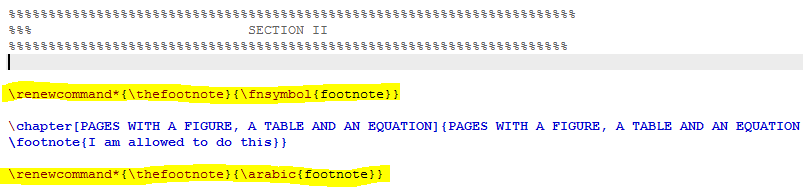
\includegraphics[scale=0.65]{Footnote.png}
	\caption{The inclusion of a copyright statement as a footnote. The lines in yellow help to change to footnote marking scheme.}
\end{figure}
			% Include the Section1.tex file
% !TEX root = ../TAMU_Thesis_Main.tex

%%%%%%%%%%%%%%%%%%%%%%%%%%%%%%%%%%%%%%%%%%%%%%%%%%%%%%%%%%%%%%%%%%%%%%%
%%%                           SECTION II
%%%%%%%%%%%%%%%%%%%%%%%%%%%%%%%%%%%%%%%%%%%%%%%%%%%%%%%%%%%%%%%%%%%%%%


\chapter{PAGES WITH A FIGURE, A TABLE AND AN EQUATION}
\section{Figures: Placement, Size, and Captions}
This is a figure template.
\begin{figure}[ht]
\centering
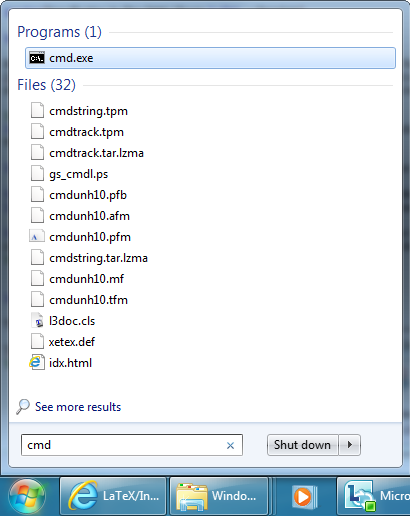
\includegraphics[scale=0.75]{TAMUthesis_CMD_windows.png}
\caption[The command line compiler in Windows.]{The command line compiler in Windows. It is not suggested that you compile using this method. See compilation instructions in the README.}

\label{fig:CMD_1}

\end{figure}

Figure (and table) titles should be consistent through the document. All captions should be placed either above or below the object it describes. This is done by placing the \textit{caption} in the correct place. While continued figures are allowed by the Thesis Manual, it is not suggested that any continued figures be included in a \LaTeX\ document. The figure below is from Linux Mint, showing a portion of a desktop.

\begin{figure}[H]
	\centering
	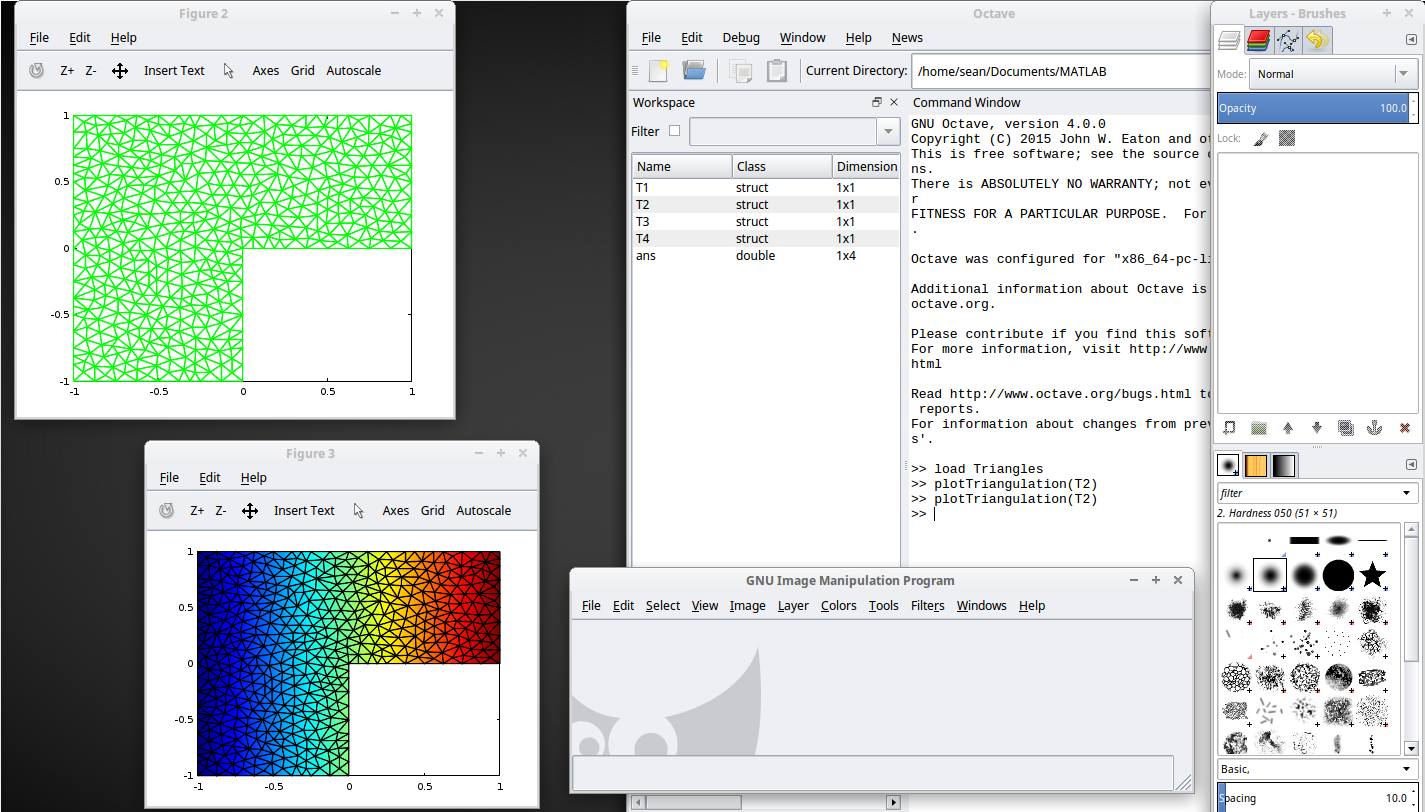
\includegraphics[width = 5.75in]{Desktop.png}
	\caption{A typical desktop space in Linux Mint.}
\end{figure}

The figure below is taken from R. While there are packages available to import graphics from R, MATLAB, and similar software, it is probably best to export plots generated by these programs as a PNG file, and then import it via the \textit{includegraphics} command.

\begin{figure}[H]
	\centering
	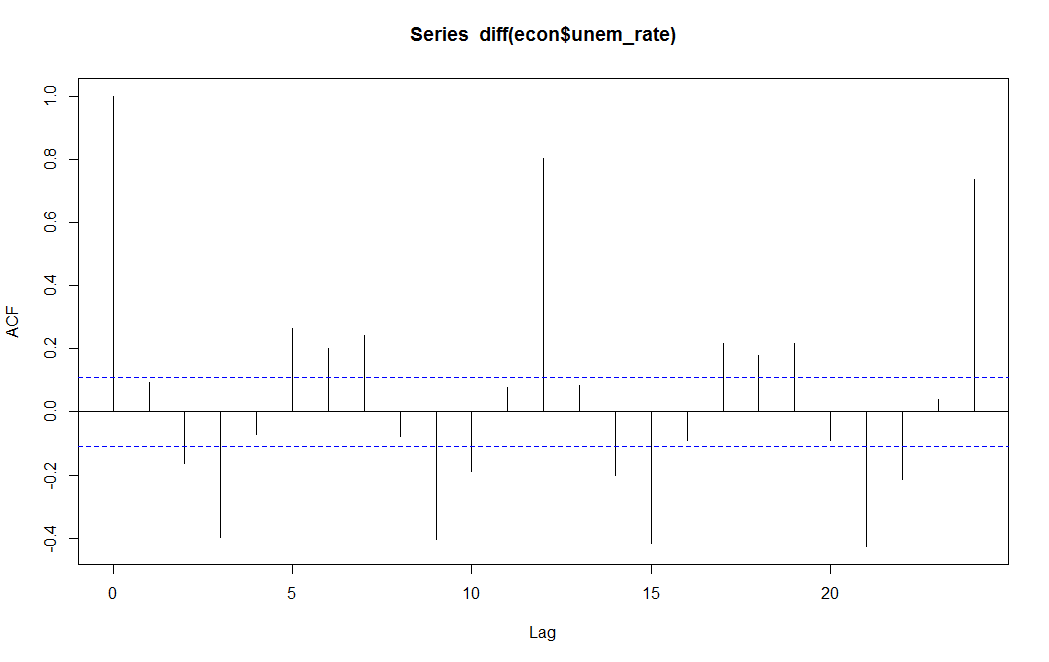
\includegraphics[scale=0.55]{UnemDiffACF.png}
	\singlespace
	\caption{The autocorrelation function (ACF) of the differenced unemployment series. Seasonal adjustments may be needed.}
\end{figure}

It is highly suggested that you scale the figures so that they fit within the margins. Almost all the figures included in this document for the sake of example have been scaled. It is best to use PNG and JPEG files as figures.

The last figure here is a screenshot from the Linux terminal.

\begin{figure}[H]
	\centering
	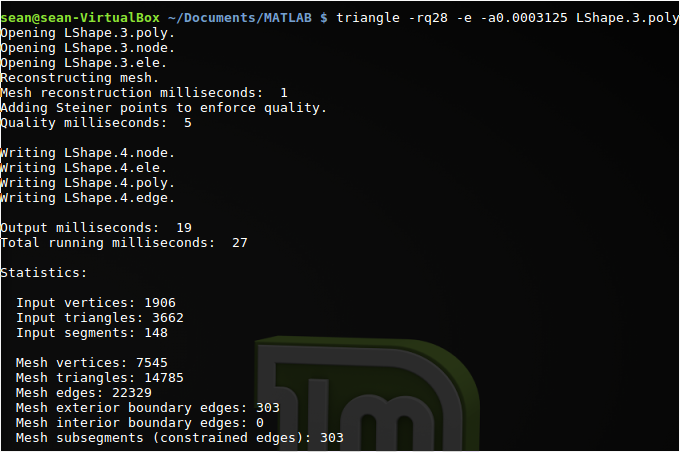
\includegraphics[width=4.75in]{Terminal1.png}
	\caption{The Linux terminal. The commands shown are from a two-dimensional mesh generator that triangulates a domain in the plane. Files containing nodes, elements, the polygon, and the edges are created.}
\end{figure}

\section{Table Placement, Size and Table Title}

Here is a table, displaying band and auxiliary scores from the 2011 Arcadia Festival of Bands held in Arcadia, CA \cite{ARCADIA}.

\begin{table}[h!]
	\centering

	\label{Band}
	\begin{tabular}{|l|l|l|}
		\hline
		School Name & Band Score & Auxiliary Score \\ \hline
		Rancho Bernardo & 96.15 & 89.15 \\ \hline
		Mt. Carmel & 95.30 & 83.55 \\ \hline
		Riverside King & 93.85 & 91.75 \\ \hline
		Diamond Bar & 93.20 & 88.60 \\ \hline
		El Dorado & 92.80 & 95.45 \\ \hline
		Chino & 92.65 & 91.45 \\ \hline
		Henry J. Kaiser & 92.60 & 87.55 \\ \hline
		Glendora & 92.60 & 89.15 \\ \hline
		Montebello & 90.50 & 82.70 \\ \hline
		Mira Mesa & 89.65 & 91.50 \\ \hline
	\end{tabular}
	\caption{Scores from the 2011 Arcadia Festival of Bands.}
\end{table}

The table is sorted by band score. There is more text here to demonstrate how the template handles spacing between tables and body text. Also note how the table caption is in a smaller font size than the body text.

\section{Equations}

The following format is recommended to be used to display equations.

%Make other examples.
\begin{equation} \label{Equ.2.1}
y=c_1\cos(t)+c_2\sin(t)
\end{equation}
\begin{equation} \label{Equ.2.2}
e^{it}=\cos(t)+i\sin(t)
\end{equation}

Equation \ref{Equ.2.1} is the general solution to the differential equation $y''+y=0$. In the source code, the \textit{ref} command allows you to refer to an equation by a label you created. References must be made after the equation has been created; attempting to refer to an equation before it is defined results in a question mark placeholder. Some more sample equations are below. Notice the first set below is not numbered.
%%
\begin{align*}
\log (x^n) &= \log (x \cdot x \cdot \ldots \cdot x) \\
&= \log x + \log x + \ldots + \log x \\
&= n \log x
\end{align*}
\begin{equation} \label{Equ.2.3}
X^T X \mathbf{u} = X^T \mathbf{y}
\end{equation}
\begin{equation}\label{Equ.2.4}
u(x, t) = \int_{-\infty}^{\infty} G(x, \tau) \exp\left(-\frac{(t-\tau)^2}{4kt}\right) \ d\tau
\end{equation}
\begin{gather}
\mathcal{L}(f) = \int_{0}^{\infty} e^{-st} f(t) \ dt \\
\begin{split} \label{Equ.2.5}
\mathcal{F}(f) = \frac{1}{2\pi}\int_{-\infty}^{\infty} e^{i \omega x} f(x) \ dx
\end{split}
\end{gather}

You can use labels to refer to equations you create. \ref{Equ.2.5} is the \textbf{Laplace transform} used extensively in differential equations. \ref{Equ.2.3} is the matrix representation of the \textbf{normal equations} used in least-squares regression.

To have equations without labels appearing the right margin, simply add an asterisk to the name of the environment (equation, align, etc.) when making the declaration.


\section{Theorems and Proofs: Examples}

This section will show an example usage of the theorem and proof environments, typically used for mathematics students. To use these environments, you must have the package \textbf{amsthm} declared in the preamble of your document. For this template, this is already declared in the main file. You may choose to remove this declaration if your document will not make use of theorems and proofs.

Theorems can be numbered, as the one below is, or you can force a different label to appear. For example, you can state the Bolzano-Weierstass theorem and have the names appear as the theorem label. See the examples below.

Sometimes you may have a theorem with multiple parts or multiple conditions. You can use other list environments, such as enumerate, inside the theorem environment declared to list these conditions. The final example at the end of this block shows this with the Invertible Matrix Theorem, which has several equivalent statements.

\newtheorem{thm}{Theorem}
\begin{thm}
	Suppose $f$ is of class $\mathcal{C}^1$ and $g$ is of class $\mathcal{C}^2$, and that the compact set $D$ and its boundary satisfy the hypotheses of Green's Theorem.  Then
	\[ \iint \limits_D f\nabla^2 g \ dA = \oint_{\partial D} f(\nabla g) \cdot \mathbf{n} \ ds - \iint \limits_D \nabla f \cdot \nabla g \ dA . \]
\end{thm}

\begin{proof}
	Begin with the integral of $f\nabla g \cdot n$ taken over the boundary of D.  By the second vector form of Green's Theorem,
	\begin{align*}
	\oint_{\partial D} f\nabla g \cdot n \ ds &= \iint \limits_D \nabla \cdot (f\nabla g) \ dA \\
	&= \iint \limits_D f\nabla^2 g + \nabla f \cdot \nabla g \ dA.
	\end{align*}
	
	Rearranging yields the desired.
\end{proof}

\begin{thm}[Bolzano-Weierstrass]
	Every bounded real sequence has a convergent subsequence.
\end{thm}

\begin{thm}[Invertible Matrix Theorem\footnote{This is an incomplete list.}]
	For any square matrix $A$ with $n$ rows and columns, the following are equivalent.
	\begin{enumerate}
		\item $A$ is invertible.
		\item The equation $A\mathbf{x}=\mathbf{0}$ has only the trivial solution $\mathbf{x} = \mathbf{0}.$
		\item For any nonzero $\mathbf{b}, \ A\mathbf{x} = \mathbf{b}$ has exactly one solution.
		\item The columns of $A$ form a linearly independent set.
		\item Zero is not an eigenvalue of $A$.
		\item $A$ has full rank.
		\item The determinant of $A$ is not zero.
	\end{enumerate}
\end{thm}

There is currently no set format on how propositions and theorems should be laid out in the document. The idea is to remain consistent. It is best to not customize the appearance of theorems so that they can easily be distinguished from body text - just like figures, tables, and headings.

\section{Another Table Example}
For the sake of testing the appearance of the list of tables, a second table will be displayed here. This table displays a list of some major universities and their enrollments during fall 2015. This table is sorted in descending order of enrollment.
%The savenotes environment, loaded from the footnote package
%(which in turn is loaded from mdwtools)
%allows you to use footnotes in tables, if needed.
\begin{savenotes}
\begin{table}[h!]
	\centering
	\label{my-label}
	\begin{tabular}{|l|l|l|}
		\hline
		School & City and State & Fall 2015 Enrollment  \\ \hline
		Texas A\&M University\footnote{Gig 'em!} & College Station, TX & 64,376  \\ \hline
		Ohio State University\footnote{This number describes enrollments at the Columbus campus; enrollments at regional campuses in Lima, Mansfield, Marion, Newark, and Wooster are not counted.} & Columbus, OH & 58,322 \\ \hline
		Iowa State University & Ames, IA & 36,001 \\ \hline
		University of California, San Diego & La Jolla, CA & 33,735   \\ \hline
		University of West Florida & Pensacola, FL & 12,798 \\ \hline
		Massachusetts Institute of Technology & Cambridge, MA & 11,319   \\ \hline
	\end{tabular}
	\caption{Some major universities and their fall 2015 enrollments.}
\end{table}
\end{savenotes}

Naturally, tables and footnotes do not go together. If you attempted to write a footnote inside a table, there will be nothing at the bottom of the page, yet the footnote marker will still appear. To remedy this, the \textit{footnote} package has been loaded from the \textit{mdwtools} package. Check your TeX distribution to see if \textit{mdwtools} is installed. See the source code for how this is implemented.

Here are some blank floats.

\begin{figure}[!h]
	\caption{A blank float.}
\end{figure}

\begin{figure}[!h]
	\caption{Another blank float.}
\end{figure}			% Include the Section2.tex file
% !TEX root = ../TAMU_Thesis_Main.tex

%%%%%%%%%%%%%%%%%%%%%%%%%%%%%%%%%%%%%%%%%%%%%%%%%%%%%%%%%%%%%%%%%%%%%%
%%                           SECTION III
%%%%%%%%%%%%%%%%%%%%%%%%%%%%%%%%%%%%%%%%%%%%%%%%%%%%%%%%%%%%%%%%%%%%%

\chapter{VERY, VERY, VERY LONG TITLE THAT FLOWS INTO A SECOND LINE FOR THE SAKE OF EXAMPLE}

Notice that the title of this section is long - much longer than the others. When you have long section titles, this template takes care of double spacing the lines in the title. If the title is long to fit in the table of contents, the template will single space the title.

\section{Yet Another Table}

Another table is placed here to show the effect of having tables in multiple sections. The list of tables should still double space between table titles, while single spacing long table titles.

%Fix table labeling.
\begin{table}[h!]
	\centering
	\begin{tabular}{|l|l|}
		\hline
		Dates & Attendance  \\ \hline
		August 8-10, 2008 & 3,523  \\ \hline
		August 14-16, 2009 & 4,003 \\ \hline
		July 9-11, 2010 & 5,049 \\ \hline
		August 5-7, 2011 & 6,891  \\ \hline
		August 10-12, 2012 & 9,464  \\ \hline
		August 16-18, 2013 & 11,077  \\ \hline
		July 18-20, 2014 & 14,686 \\ \hline
		July 31-August 2, 2015 & 18,411  \\ \hline
	\end{tabular}
	\caption{San Japan attendance. Data is taken from \cite{ANCONS}. I intentionally make the title of this table long so the single space effect is seen in the list of tables.}
\end{table}

You may be wondering why San Japan was chosen. There are a few reasons as to why I did this:

\begin{enumerate}
\item It is one of the fastest-growing anime conventions in Texas.
\item Filler.
\item I wanted a good variety of table examples.
\item Because conventions are cool.
\end{enumerate}

The \textit{enumerate} environment was used to generated an ordered list above.

\section{Section Test Example}
We insert another figure here, just for kicks.

\begin{figure}[h!]
	\centering
	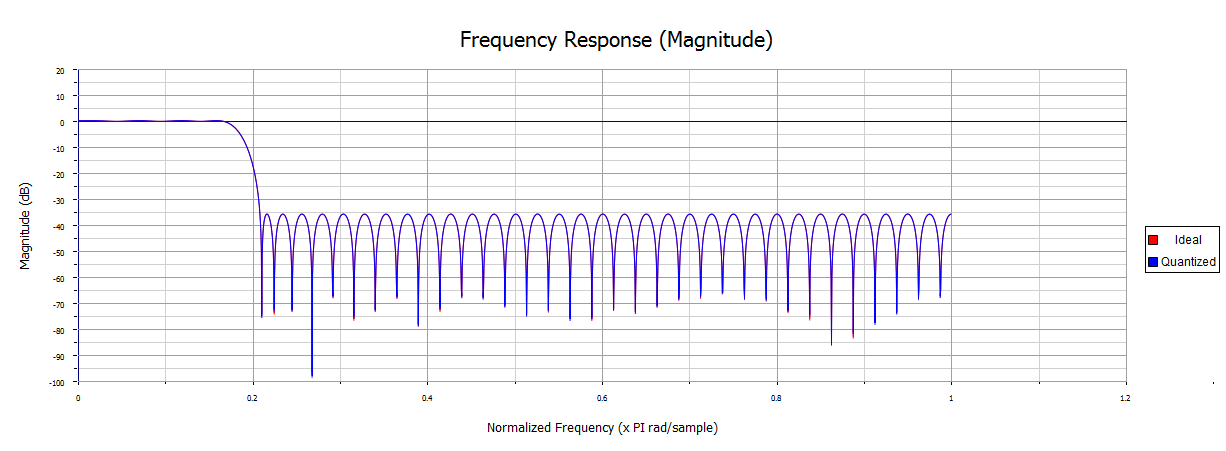
\includegraphics[width = 6.0in]{LowPass_Filter_Design.png}
	\caption{A low pass filter design.}
\end{figure}

\subsection{Filler, Filler, Filler}

This section has filler text. These words serve no meaning except to fill a few lines in the document. This section has filler text. These words serve no meaning except to fill a few lines in the document. This section has filler text. These words serve no meaning except to fill a few lines in the document.

\begin{figure}[h!]
	\centering
	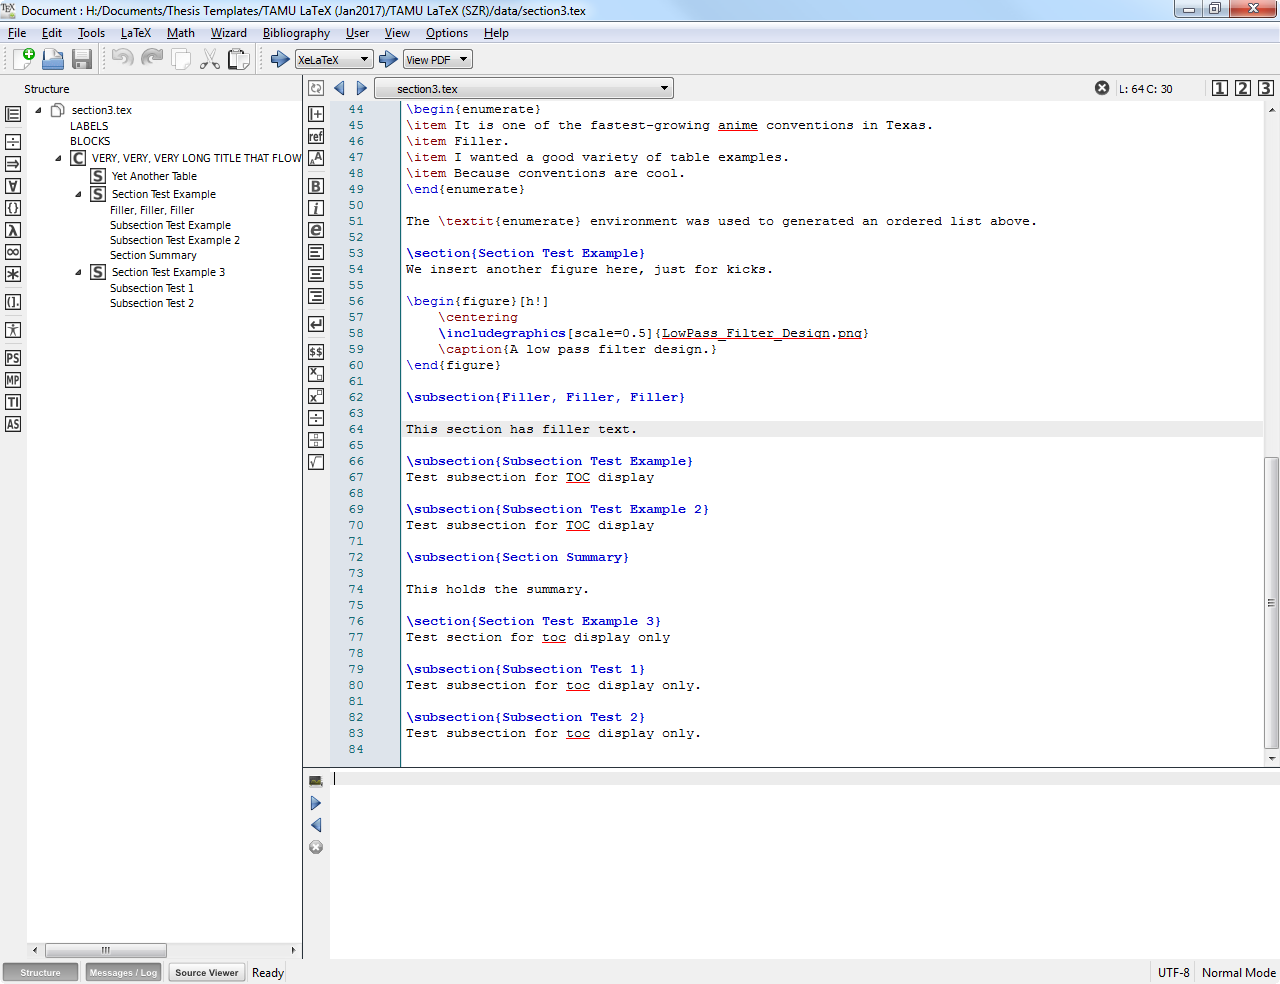
\includegraphics[width=3.75in]{Workspace1.png}
	\caption{A typical Texmaker workspace in Windows 7. The right sidebar displays the current file's structure according to the subsections in place.}
\end{figure}

This section has filler text. These words serve no meaning except to fill a few lines in the document. This section has filler text. These words serve no meaning except to fill a few lines in the document. This section has filler text. These words serve no meaning except to fill a few lines in the document. This section has filler text. These words serve no meaning except to fill a few lines in the document. This section has filler text. These words serve no meaning except to fill a few lines in the document. This section has filler text. These words serve no meaning except to fill a few lines in the document.

\begin{figure}[h!]
	\centering
	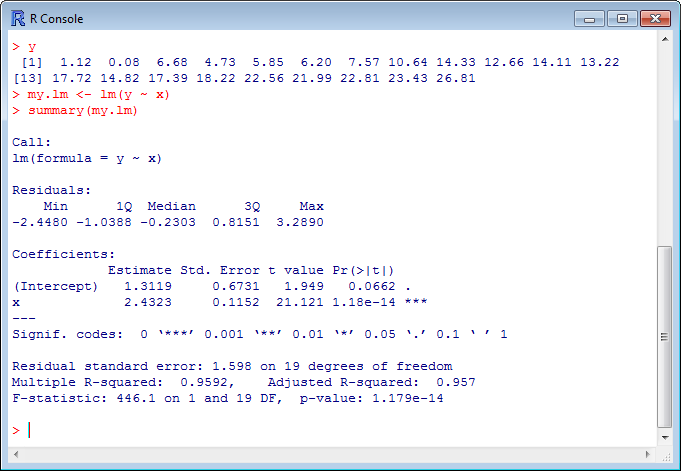
\includegraphics[width=3.5in]{Rachl1.png}
	\caption{Some commands in R.}
\end{figure}

\subsection{Subsection Test Example}
Test subsection for TOC display

\subsection{Subsection Test Example 2}
This section has filler text. These words serve no meaning except to fill a few lines in the document. This section has filler text. These words serve no meaning except to fill a few lines in the document. This section has filler text. These words serve no meaning except to fill a few lines in the document.

\begin{figure}[h!]
	\centering
	
\includegraphics[scale=0.85]{TAM_Logo1.png}
	\caption{The logo of a familiar university.}
\end{figure}

\begin{figure}[!h]
	\caption{Yet another blank float that has no purpose. This is only to test the appearance of the Lists of Figures and the List of Tables.}
\end{figure}

\subsection{Section Summary}
  
This holds the summary. Well, not really a summary - there was a lot of filler in this section.

\begin{figure}[h!]
	\centering
	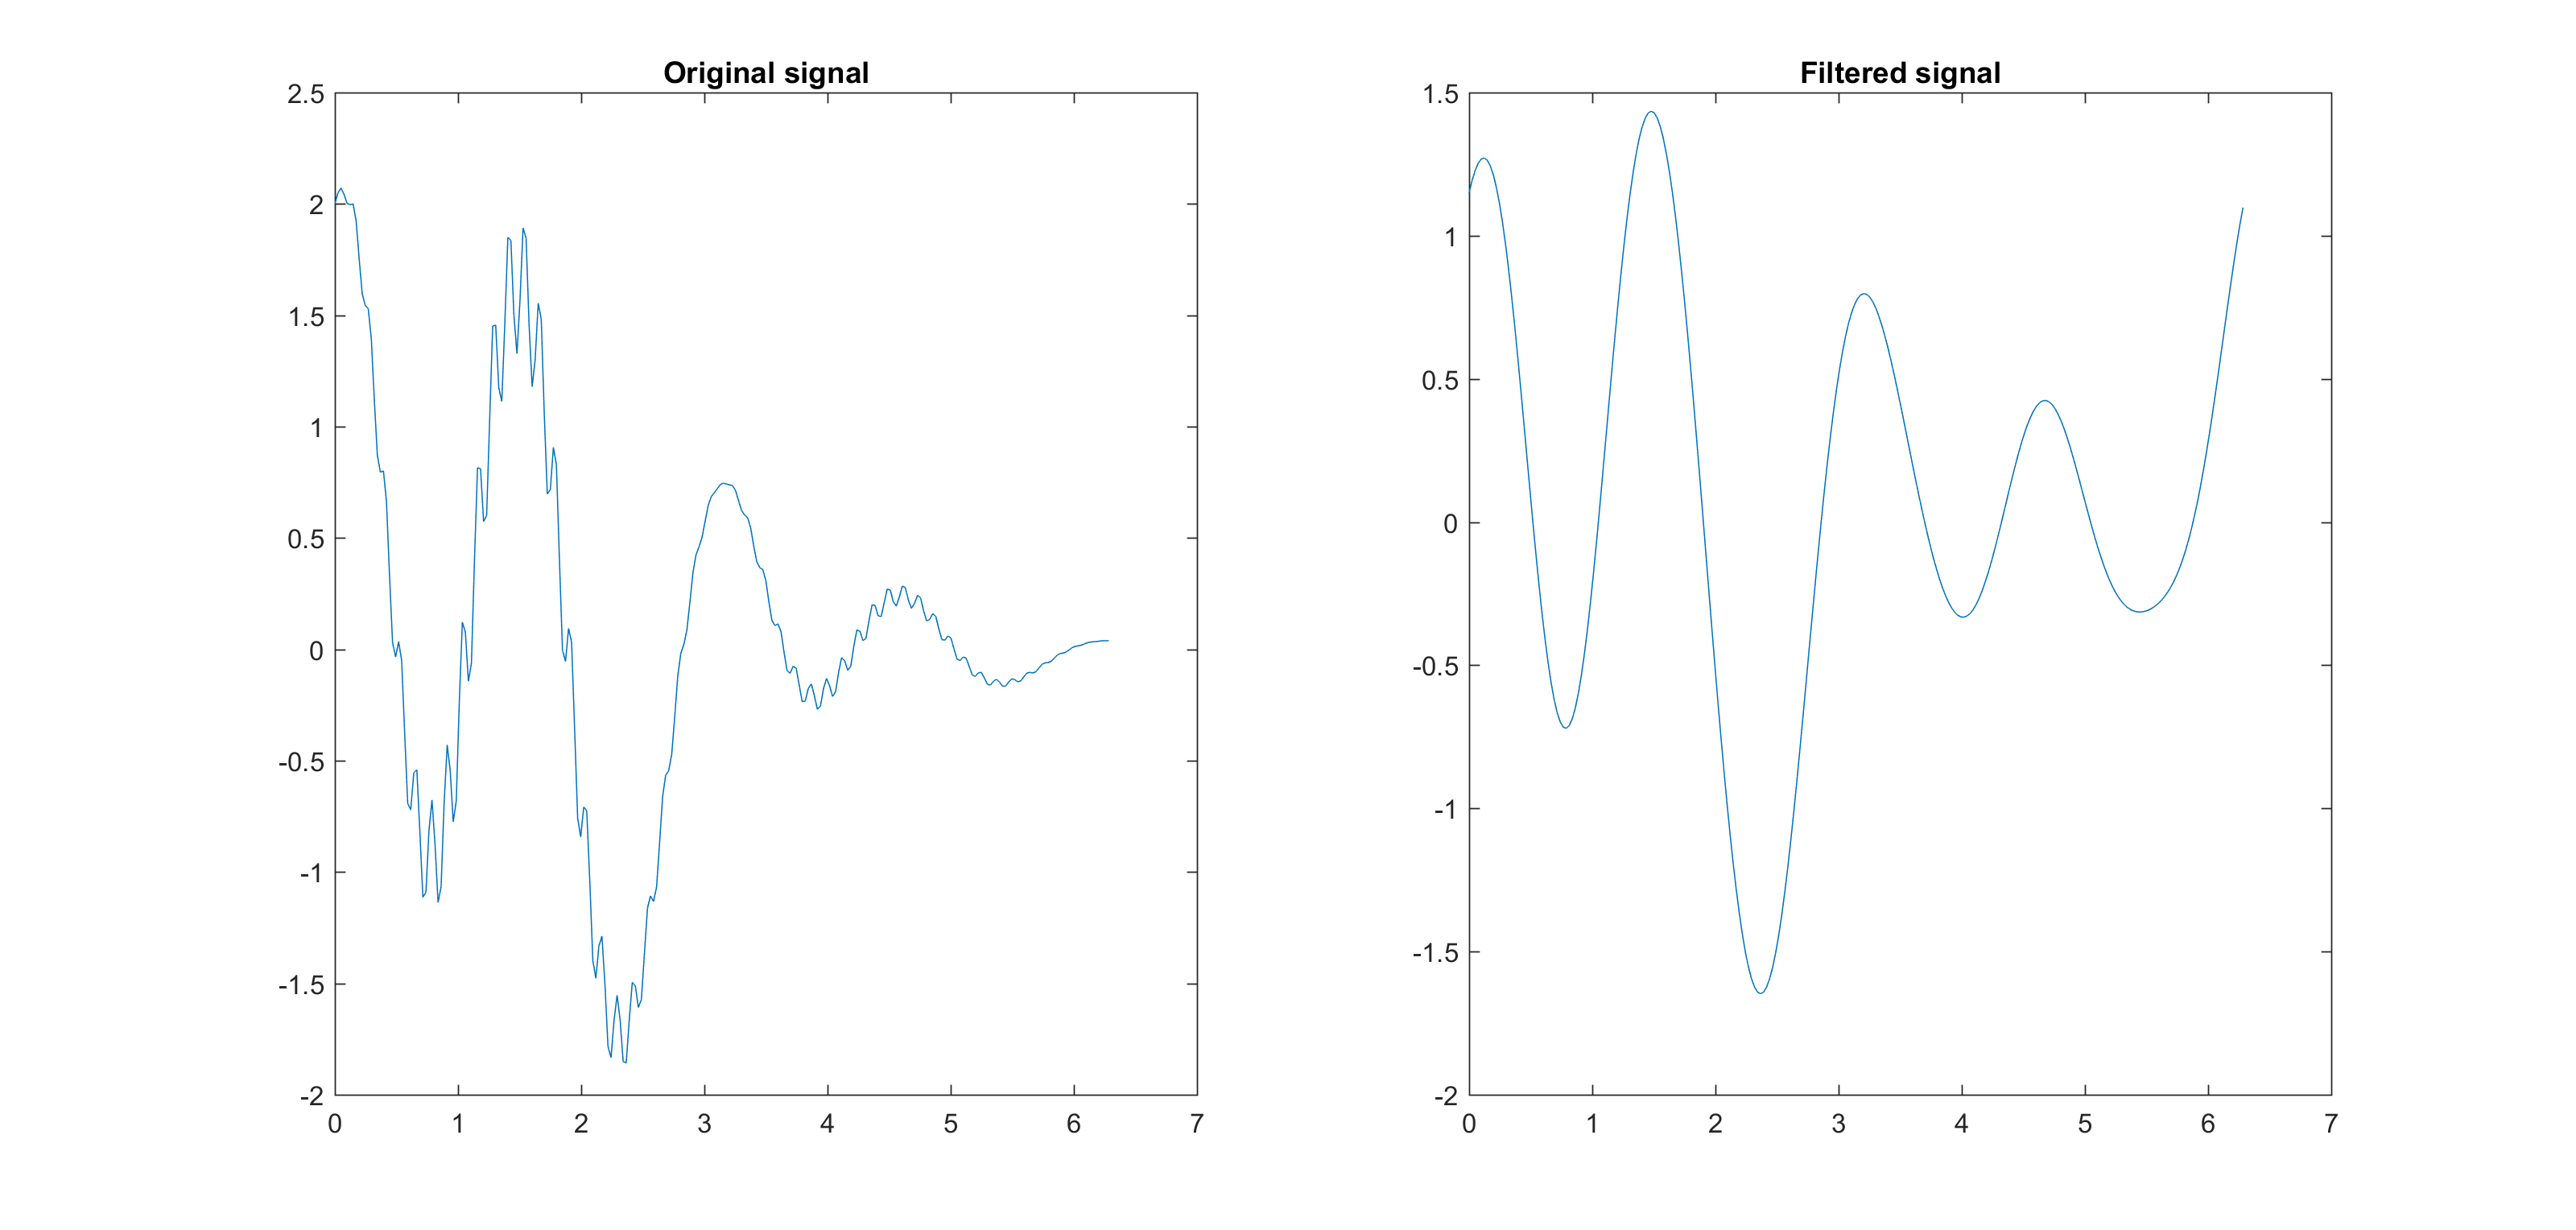
\includegraphics[width=6.5in]{Filter1.png}
	\caption{A signal and the result after a basic filter. The FFT was used to create the plot on the right.}
\end{figure}

\section{Section Test Example 3}
Test section for toc display only.

\begin{figure}[!h]
	\caption{There is nothing to see here.}
\end{figure}

\begin{figure}[!h]
	\caption{There is another float here. I wonder what could be here? Guess what? Nothing! There is no material in this float.}
\end{figure}

\subsection{Subsection Test 1}
Test subsection for toc display only.

\subsection{Subsection Test 2}
Test subsection for toc display only.			% Include the Section3.tex file
% !TEX root = ../TAMU_Thesis_Main.tex
%%%%%%%%%%%%%%%%%%%%%%%%%%%%%%%%%%%%%%%%%%%%%%%%%%%
%
%  New template code for TAMU Theses and Dissertations starting Fall 2016.
%
%  Author: Sean Zachary Roberson
%	 Version 3.16.09
%  Last updated 9/12/2016
%
%  Modified 04 Nov. 2016 by Kyle R. Wodzicki
%%%%%%%%%%%%%%%%%%%%%%%%%%%%%%%%%%%%%%%%%%%%%%%%%%%
%%%%%%%%%%%%%%%%%%%%%%%%%%%%%%%%%%%%%%%%%%%%%%%%%%%%%%%%%%%%%%%%%%%%%%
%%                           SECTION IV
%%%%%%%%%%%%%%%%%%%%%%%%%%%%%%%%%%%%%%%%%%%%%%%%%%%%%%%%%%%%%%%%%%%%%



\chapter{SUMMARY AND CONCLUSIONS}\label{cha:Summary}

**Some text/figure here**

\section{Challenges}
Section here is to test toc display only.

\section{Further Study}
Section here is to test toc display only.

			% Include the Section4.tex file

%%%%%%%%%%%%%%%%%%%%%%%%%%%%%%%%%%%%%%%%%%%%%%%%%%%%
% Generate the Bibliography
% MUST BE IN BIBLIOGRAPHY ENVIRONMENT!!!
\begin{references}
	\bibliographystyle{ieeetr}			% Set the bibliography style
	\bibliography{myReference}			% Set path to bibliography .bib file
\end{references}

%%%%%%%%%%%%%%%%%%%%%%%%%%%%%%%%%%%%%%%%%%%%%%%%%%%%
% Include appendices. 
% MUST BE IN APPENDICES ENVIRONMENT!!!
\begin{appendices}
	% !TEX root = ../TAMU_Thesis_Main.tex
%%%%%%%%%%%%%%%%%%%%%%%%%%%%%%%%%%%%%%%%%%%%%%%%%%%
%
%  New template code for TAMU Theses and Dissertations starting Fall 2016.
%
%
%  Author: Sean Zachary Roberson 
%	 Version 3.16.09
%  Last updated 9/12/2016
%
%  Modified 04 Nov. 2016 by Kyle R. Wodzicki
%%%%%%%%%%%%%%%%%%%%%%%%%%%%%%%%%%%%%%%%%%%%%%%%%%%

%%%%%%%%%%%%%%%%%%%%%%%%%%%%%%%%%%%%%%%%%%%%%%%%%%%%%%%%%%%%%%%%%%%%%%
%%                           APPENDIX A 
%%%%%%%%%%%%%%%%%%%%%%%%%%%%%%%%%%%%%%%%%%%%%%%%%%%%%%%%%%%%%%%%%%%%%

%\phantomsection

\chapter{First Appendix}\label{appendix:01}

Text for the Appendix follows.

\begin{figure}[h]
\centering
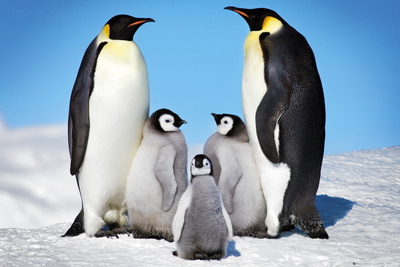
\includegraphics[scale=.50]{figures/Penguins.jpg}
\caption{TAMU figure}
\label{fig:tamu-fig5}
\end{figure}
			% Include the appendix1.tex file
	%%%%%%%%%%%%%%%%%%%%%%%%%%%%%%%%%%%%%%%%%%%%%%%%%%%
%
%  New template code for TAMU Theses and Dissertations starting Fall 2012.  
%  For more info about this template or the 
%  TAMU LaTeX User's Group, see http://www.howdy.me/.
%
%  Author: Wendy Lynn Turner 
%	 Version 1.0 
%  Last updated 8/5/2012
%
%%%%%%%%%%%%%%%%%%%%%%%%%%%%%%%%%%%%%%%%%%%%%%%%%%%

%%%%%%%%%%%%%%%%%%%%%%%%%%%%%%%%%%%%%%%%%%%%%%%%%%%%%%%%%%%%%%%%%%%%%%
%%                           APPENDIX B
%%%%%%%%%%%%%%%%%%%%%%%%%%%%%%%%%%%%%%%%%%%%%%%%%%%%%%%%%%%%%%%%%%%%%

\chapter{\uppercase {Second Appendix with a longer title - much longer in fact}}

Text for the Appendix follows.

\begin{figure}[H]
\centering
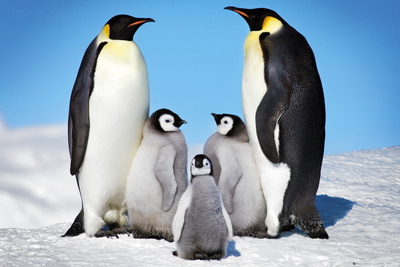
\includegraphics[scale=.50]{figures/Penguins.jpg}
\caption{TAMU figure}
\label{fig:tamu-fig6}
\end{figure}

\section{Appendix Section}


\pagebreak{}			% Include the appendix2.tex file
	% !TEX root = ../TAMU_Thesis_Main.tex
%%%%%%%%%%%%%%%%%%%%%%%%%%%%%%%%%%%%%%%%%%%%%%%%%%%
%
%  New template code for TAMU Theses and Dissertations starting Fall 2016.
%
%
%  Author: Sean Zachary Roberson 
%	 Version 3.16.09 
%  Last updated 9/12/2016
%
%  Modified 04 Nov. 2016 by Kyle R. Wodzicki
%%%%%%%%%%%%%%%%%%%%%%%%%%%%%%%%%%%%%%%%%%%%%%%%%%%

%%%%%%%%%%%%%%%%%%%%%%%%%%%%%%%%%%%%%%%%%%%%%%%%%%%%%%%%%%%%%%%%%%%%%%
%%                           APPENDIX B
%%%%%%%%%%%%%%%%%%%%%%%%%%%%%%%%%%%%%%%%%%%%%%%%%%%%%%%%%%%%%%%%%%%%%

\chapter{Bibliography Information}\label{appendix:02}

As previously mentioned, one program that can be used to organize references is \href{http://www.jabref.org}{\textbf{JabRef}}. While a tutorial of how to use \textbf{JabRef} is beyond the scope of this template, a brief discussion of how to use \textbf{BibTeX} follows.

\section{BibTeX}
After you have installed \textbf{JabRef}, or any citation manager of your choosing that is compatible with \textbf{BibTeX}, you must create a \textbf{BibTeX} database. This database file will contain all the information \textbf{BibTeX} requires to generate your bibliography. An example .bib file named `myReference.bib' is included in this template. The first entry of that file is shown below.

{\footnotesize \begin{verbatim}
@Article{Barn-JORVQ,
  author  = {Christopher F. Barnes and Richard L. Frost},
  title   = {Residual Vector Quantizers with Jointly Optimized Code Books},
  journal = {Advances in Electronics and Electron Physics},
  year    = {1992},
  volume  = {84},
  pages   = {1--59},
}
\end{verbatim}}

All of the entries in the entry are very self-explanatory, such as author and title, however, arguably the most important part of the entry is the key. The key is the first value after @Article, which is Barn-JORVQ in this example. This is the key you will use in any cite commands for references, e.g.,

{\footnotesize\begin{verbatim}\cite{Barn-JORVQ}\end{verbatim}}.


Depending on the citation style that is used, there may be different cite commands for different types of in-text citations. It is important to know which commands must be used with the citation style you are using.

\section{Compiling with BibTeX}
When compiling your \LaTeX{} document, it is also important to remember to compile it twice to ensure that all equation, fig, table, etc. cross-references have updated correctly. However, when using citations from a .bib file in your document, the process is a little longer. To ensure that your bibliography generates correctly, one must run XeLaTeX, then BibTeX, then XeLaTeX twice. This will ensure that all the citations and cross-references are updated correctly. If you are using a program such as \textbf{MikTeX} or \textbf{ProTeXt}, this may be the default compilation method. However, if you use \textbf{TeXShop} on a Mac, you must change the compiler manually. If compiling from command line, the sequence would be:

{\footnotesize \begin{verbatim}
xelatex TAMU_Thesis_Main.tex
bibtex TAMU_Thesis_Main.aux
xelatex TAMU_Thesis_Main.tex
xelatex TAMU_Thesis_Main.tex
\end{verbatim}}

Be sure to check the output for any errors. If question marks (?) appear in any location where a reference should be, there was an issue with the compilation. Make certain that the key used in the cite command matches the corresponding references in the .bib file.

\section{References at the end of chapters}
If you would like references at the end of each chapter, first make sure you are using the `chapref' options in the documentclass command at the top of the Main \LaTeX document. Once that option is set, compilation is similar to the method discussed above.

First, compile the main file use XeLaTeX. When it is done compiling, check the directory your document is saved in. There should be a bunch of files named `bu*.aux', where the asterisk represents any number. You will now want to run bibtex on all of these .aux files as well as the .aux file from the main document. After bibtex is run on all the .aux files, run XeLaTeX two more times and your document should be good to go! If you are on a Mac, open up a Terminal window, cd into the directory your document is in and run the following commands (should work on any Linux machine as well):

{\footnotesize \begin{verbatim}
xelatex TAMU_Thesis_Main.tex
find ./ -name '*.aux' -exec bibtex '{}' \;
xelatex TAMU_Thesis_Main.tex
xelatex TAMU_Thesis_Main.tex
\end{verbatim}}
The second command simply finds all the .aux files in the current working directory and executes (exec) the command bibtex on each of them.

Be sure to check the output for any errors. If question marks (?) appear in any location where a reference should be, there was an issue with the compilation. Make certain that the key used in the cite command matches the corresponding references in the .bib file.			% Include the appendix3.tex file
\end{appendices}

\end{document}